
\section{Neural Bayesian Learning}
\frame{Neural Bayesian Learning (NBL): \\
Robust Data-Driven Stochastic Control Design}

\begin{frame}[fragile]{Completed Work}

  \begin{columns}
    \begin{column}{0.58\linewidth}
      \begin{exampleblock}{Neural Bayesian Learning}
        \begin{equation*}
          \begin{aligned}
              \underset{q(\theta) }{\text{min}} 
              &&\quad J(&\phi(t; x_0, u), u) \\
              \text{subject to} 
              &&\quad \dd {x} &= f(x, u; \zeta) \dd t + \nabla_x u(x) \dd W_t, \\
              &&\quad u(x; \theta) &= \mathcal{D} \{F(x; \theta) \}, \\
              &&\quad \zeta &\sim \mathcal{N}(\zeta_0, \Sigma_\zeta), \\
              &&\quad \theta &\sim q(\theta).
          \end{aligned}    
        \end{equation*}
      \end{exampleblock}
      \begin{itemize}
        \item $F(x;\theta)$ is a \textit{Bayesian neural network}.
        \item $\phi(t;x_0, u)$ is a trajectory generated from policy $u$ starting at initial state $x_0$.
        \item $\zeta$ is a vector of system parameters with uncertainties $\Sigma_\zeta$.
        % \item The closed-form solution to the optimization problem is intractable.
      \end{itemize}
    \end{column}
    \begin{column}{0.42\linewidth}
      \centering
      % ~
      \resizebox{0.7\textwidth}{!}{%
      \begin{tikzpicture}[
        shorten >=1pt,->,draw=black!70, node distance=\layersep,
        neuron/.style={circle,fill=black!25,minimum size=20,inner sep=0},
        edge/.style 2 args={pos={(mod(#1+#2,2)+1)*0.33}, font=\tiny},
        distro/.style 2 args={
            edge={#1}{#2}, node contents={}, minimum size=0.6cm, path picture={\draw[double=orange,white,thick,double distance=1pt,shorten >=0pt] plot[variable=\t,domain=-1:1,samples=51] ({\t},{0.2*exp(-100*(\t-0.05*(#1-1))^2 - 3*\t*#2))});}
        },
        weight/.style 2 args={
            edge={#1}{#2}, node contents={\pgfmathparse{0.35*#1-#2*0.15}\pgfmathprintnumber[fixed]{\pgfmathresult}}, fill=white, inner sep=2pt
        }
      ]
        \nn{regular}
        % Draw weights for all regular edges.    
        \foreach \i in {1,...,2}
            \foreach \j in {1,...,4}
                \path (i\i-regular) -- (h\j-regular) node[weight={\i}{\j}];
        \foreach \i in {1,...,4}
            \path (h\i-regular) -- (o-regular) node[weight={\i}{1}];
    
      \end{tikzpicture}
      }

      ~

      \resizebox{0.7\textwidth}{!}{%
      \begin{tikzpicture}[
        shorten >=1pt,->,draw=black!70, node distance=\layersep,
        neuron/.style={circle,fill=black!25,minimum size=20,inner sep=0},
        edge/.style 2 args={pos={(mod(#1+#2,2)+1)*0.33}, font=\tiny},
        distro/.style 2 args={
            edge={#1}{#2}, node contents={}, minimum size=0.6cm, path picture={\draw[double=orange,white,thick,double distance=1pt,shorten >=0pt] plot[variable=\t,domain=-1:1,samples=51] ({\t},{0.2*exp(-100*(\t-0.05*(#1-1))^2 - 3*\t*#2))});}
        },
        weight/.style 2 args={
            edge={#1}{#2}, node contents={\pgfmathparse{0.35*#1-#2*0.15}\pgfmathprintnumber[fixed]{\pgfmathresult}}, fill=white, inner sep=2pt
        }
      ]
        \nn{bayes}
        % Draw distros for all Bayesian edges.
        \foreach \i in {1,...,2}
            \foreach \j in {1,...,4}
                \path (i\i-bayes) -- (h\j-bayes) node[distro={\i}{\j}];
        \foreach \i in {1,...,4}
            \path (h\i-bayes) -- (o-bayes) node[distro={\i}{1}];
      \end{tikzpicture}
      }
    \end{column}
  \end{columns}

\end{frame}


\begin{frame}{}
  \begin{algorithm}[H]
    \centering
    \small
    % \setstretch{1.0}
    \caption{Neural Bayesian Learning}
    \begin{algorithmic}
      \algrenewcommand\algorithmicindent{0em} % No indent
      \onslide<1->{
        \color{gray}
        \only<1>{\color{black}}

        \State Select a prior distribution $p(\theta)$
        \State $f \,\gets f(x, u^\theta; \zeta)$ dynamics given by SDE using current policy $u^\theta$
        \State $\mathcal{D} \gets \{x_0\}_{(N_{\mathcal{D}})}$  \Comment{$N_{\mathcal{D}}$ samples of $x_0$}
      }
      
      \algrenewcommand\algorithmicindent{1.5em} % Change indent back to default

      \onslide<1->{
        \color{gray}
        \only<2>{\color{black}}
        \For{$i=1:\texttt{maxiters}$}
          \For{each $d$ $\subset \mathcal {D}$} \Comment Select batch $d$ from dataset $\mathcal{D}$
              \State Initialize $\mathcal{J} = 0$
              \State $\theta \sim  q(\theta ; z)$ \Comment{Sample parameters of $F$ from posterior}
      }

      \onslide<1->{
        \color{gray}
        \only<3>{\color{black}}

        \For{each $x_0 \in d$}
            \State $\zeta \sim \mathcal{N}(\zeta_0,\Sigma_{\zeta})$ \Comment{Sample system parameters}
            \State $\phi(t; x_0, u^\theta) \gets$ integrate dynamics from $x_0$ 
            \State $\mathcal{J} \gets \mathcal{J} + J(\phi(t; x_0, u^\theta), u^\theta)$
        \EndFor
        \State Compose likelihood $p(d | \theta)$
        \State Compute \textsc{Elbo} $\mathcal{L}(J,z) = \mathbb{E}_{\theta \sim q} \left[\log( p(J \mid \theta;z)p(\theta;z)) - \log(q(\theta;z)) \right]$
        \State $z \leftarrow  z + \alpha \; \partial \mathcal{L} / \partial z$
        \EndFor
      }

      \onslide<1->{
        \color{gray}
        \only<4>{\color{black}}
        \State $\mathcal{D} \gets \{\mathcal{D}\}_{(1,\ldots,N_{\mathcal{D}}-N_{\textrm{R}})} \cup \{x_0\}_{(N_{\textrm{R}})}$\Comment{Replay buffer}
      \EndFor
      
      \State \textbf{return} $q(\theta; z)$
      }
    \end{algorithmic}
    \addtocounter{algorithm}{-1}
  \end{algorithm}
\end{frame}

% \begin{frame}{Gradient of \textsc{Elbo}}
%   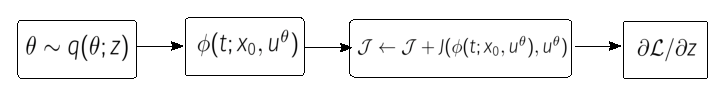
\includegraphics[width = 0.9\linewidth]{gradient.eps}
%   \begin{itemize}
%     \item Automatic differentiation techniques are used to compute gradients through the stochastic differential equations.
%   \end{itemize}
% \end{frame}
